% Author: Izaak Neutelings (October 2020)
\documentclass[border=3pt,tikz]{standalone}
\usepackage{physics}
\usepackage{siunitx}
\usepackage{tikz,pgfplots}
%\usepackage[outline]{contour} % glow around text
\usetikzlibrary{calc}
\usetikzlibrary{angles,quotes} % for pic
\usetikzlibrary{arrows.meta}
\tikzset{>=latex} % for LaTeX arrow head
%\contourlength{1.4pt}

\colorlet{xcol}{blue!60!black}
\colorlet{vcol}{green!60!black}
\colorlet{myred}{red!65!black}
\colorlet{myblue}{blue!70!black}
\colorlet{mygreen}{green!40!black}
\colorlet{myorange}{orange!90!black}
\colorlet{mypurple}{red!50!blue!90!black!80}
\colorlet{mydarkred}{myred!70!black}
\colorlet{mydarkblue}{myblue!60!black}
\colorlet{acol}{red!50!blue!80!black!80}
\tikzstyle{CM}=[red!40!black,fill=red!80!black!80]
\tikzstyle{xline}=[xcol,thick]
\tikzstyle{mass}=[line width=0.6,red!30!black,fill=red!40!black!10,rounded corners=1,
                  top color=red!40!black!20,bottom color=red!40!black!10,shading angle=20]
\tikzstyle{faded mass}=[dashed,line width=0.1,red!30!black!40,fill=red!40!black!10,rounded corners=1,
                        top color=red!40!black!10,bottom color=red!40!black!10,shading angle=20]
\tikzstyle{rope}=[brown!70!black,very thick,line cap=round]
\def\rope#1{ \draw[black,line width=1.4] #1; \draw[rope,line width=1.1] #1; }
\tikzstyle{force}=[->,myred,very thick,line cap=round]
\tikzstyle{velocity}=[->,vcol,very thick,line cap=round]
\tikzstyle{Fproj}=[force,myred!40]
\tikzstyle{myarr}=[-{Latex[length=3,width=2]},thin]
\def\tick#1#2{\draw[thick] (#1)++(#2:0.12) --++ (#2-180:0.24)}

\begin{document}


% PENDULUM
\def\L{2.8}  % string length
\def\ang{28} % angle string
\def\R{0.25} % ball radius
\def\F{1.0}  % force magnitude
\begin{tikzpicture}
  \message{^^JPendulum}
  \coordinate (M) at (\ang-90:\L);
  \coordinate (M') at (0,-\L);
  \coordinate (O) at (0,0);
  \coordinate (B) at (0,-\L-2.2*\R);
  \coordinate (FT) at ($(M)+(90+\ang:{\F*cos(\ang)+\R})$);
  \coordinate (FG) at ($(M)+(-90:{\F+\R})$);
  \coordinate (FGx) at ($(M)+(-90+\ang:{0.55*\F+\R})$);
  \coordinate (MA) at ($(M)+(180+\ang:{\F*sin(\ang)+\R})$);
  %\draw[faded mass] (M') circle(\R);
  \draw[<->] (M)++(\ang-32:0.2*\L) node[below right=-1,scale=0.9] {$x$}
    --++ (\ang:0.17*\L) --++ (90+\ang:0.17*\L) node[above right=-1,scale=0.9] {$y$};
  \draw[dashed] (O) -- (B);
  %\draw[dashed,myred!60!black] (MA) -- (FG);
  \draw[dashed,myred!60!black] (M) -- (FGx);
  \draw[dashed] (-90+\ang+10:\L) arc(-90+\ang+10:-110:\L) (B);
  \rope{(O) -- (M)} \path (O) -- (M) node[midway,above right=-1] {$L$};
  \fill[black] (O) circle(0.04);
  \draw[force] (M) -- (FT) node[midway,left=0] {$\vb{T}$};
  \draw[force] (M) -- (FG) node[right=0] {$m\vb{g}$};
  \draw[force,acol] (M) -- (MA) node[right=2,below=0] {$m\vb{a}$}; %{\contour{white}{$m\vb{a}$}};
  \draw[mass] (M) circle(\R) node {$m$};
  \draw pic[myarr,"$\theta$",xcol,draw=xcol,angle radius=22,angle eccentricity=1.30] {angle=B--O--M}; %_\text{max}
  \draw pic[myarr,"$\theta$",xcol,draw=xcol,angle radius=14,angle eccentricity=1.45] {angle=FG--M--FGx};
\end{tikzpicture}


% PENDULUM FORCES
\begin{tikzpicture}
  \message{^^JPendulum forces}
  \def\F{1.4}  % force magnitude
  \coordinate (O) at (0,0);
  \coordinate (FT) at (90+\ang:{\F*cos(\ang)});
  \coordinate (FG) at (-90:\F);
  \coordinate (FGx) at (-90+\ang:{0.7*\F});
  \coordinate (MA) at (180+\ang:{\F*sin(\ang)});
  \draw[dashed,myred!60!black] (O) -- (FGx);
  \draw[dashed,myred!60!black] (MA) -- (FG);
  \draw[force] (O) -- (FT) node[midway,above right=-2] {$\vb{T}$};
  \draw[force] (O) -- (FG) node[right=0] {$m\vb{g}$};
  \draw[force,acol] (O) -- (MA) node[left=0] {$m\vb{a}$};
  \draw pic[myarr,"$\theta$",xcol,draw=xcol,angle radius=14,angle eccentricity=1.45] {angle=FG--O--FGx};
\end{tikzpicture}


%% PENDULUM 
%\begin{tikzpicture}
%  \coordinate (M) at (0,-\L);
%  \coordinate (O) at (0,0);
%  \rope{(O) -- (M)} \path (O) -- (M) node[midway,above right=-2] {$L$};
%  \fill[black] (O) circle(0.04);
%  \draw[velocity] (M)++(-\R,0) --++ (-2.7*\R,0) node[above=0] {$\vb{v}$};
%  \draw[mass] (M) circle(\R) node {$m$};
%\end{tikzpicture}


% PHYSICAL PENDULUM
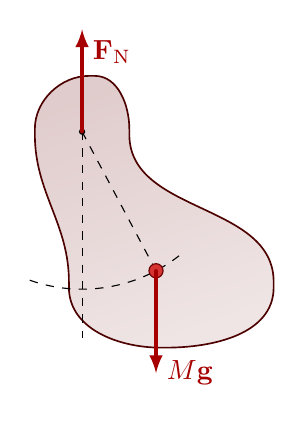
\begin{tikzpicture}
  \message{^^JPhysical pendulum}
  \def\L{2.0}  % string length
  \def\ang{28} % angle string
  \def\R{0.25} % ball radius
  \def\F{1.3}  % force magnitude
  \coordinate (M) at (\ang-90:\L);
  \coordinate (R) at (\ang-90:1.1*\L);
  \coordinate (M') at (0,-\L);
  \coordinate (O) at (0,0);
  \coordinate (B) at (0,-\L-2.5*\R);
  \coordinate (FT) at (90:\F);
  \coordinate (FG) at ($(M)+(-90:\F)$);
  \coordinate (FGx) at ($(M)+(-90+\ang:{0.55*\F+\R})$);
  \coordinate (MA) at ($(M)+(180+\ang:{\F*sin(\ang)+\R})$);
  \draw[mass]
    (180:0.3*\L) to[out=90,in=180] (80:0.36*\L) to[out=0,in=90] (0:0.3*\L) to[out=-90,in=90]
    ($(R)+(0:0.7*\L)$) to[out=-90,in=0] ($(R)+(-90:0.4*\L)$) to[out=180,in=-90] ($(R)+(-180:0.6*\L)$) to[out=90,in=-90] cycle; %node {$m$};
  \draw[dashed] (O) -- (B);
  \draw[dashed] (O) -- (M);
  %\draw[dashed,myred!60!black] (MA) -- (FG);
  \draw[dashed] (-90+\ang+10:\L) arc(-90+\ang+10:-110:\L) (B);
  \fill[black] (O) circle(0.04);
  \draw[CM] (M) circle(0.09);
  \draw[force] (O) -- (FT) node[below right=0] {$\vb{F}_\mathrm{N}$};
  \draw[force] (M) -- (FG) node[right=0] {$M\vb{g}$};
%  \draw[force,acol] (M) -- (MA) node[right=2,below=0] {$m\vb{a}$}; %{\contour{white}{$m\vb{a}$}};
%  \draw pic[myarr,"$\theta$",xcol,draw=xcol,angle radius=22,angle eccentricity=1.30] {angle=B--O--M}; %_\text{max}
%  \draw pic[myarr,"$\theta$",xcol,draw=xcol,angle radius=14,angle eccentricity=1.45] {angle=FG--M--FGx};
\end{tikzpicture}


% EXACT SOLUTION
% To compile, include data files from
%   https://github.com/IzaakWN/CodeSnippets/tree/master/LaTeX/TikZ/physics/dynamics_pendulum
% Other sources:
%   https://www.scielo.br/scielo.php?script=sci_arttext&pid=S1806-11172007000400024
%   https://www.researchgate.net/publication/262746594_Exact_solution_for_the_nonlinear_pendulum
%   https://tex.stackexchange.com/questions/545590/phase-portrait-of-van-der-pol-oscillator-with-pgfplots
%   http://matlab.cheme.cmu.edu/2011/08/09/phase-portraits-of-a-system-of-odes/
\begin{tikzpicture}
  \message{^^JPendulum exact solution}
  \def\xmax{7.0}     % max x axis
  \def\ymax{1.4}     % max y axis
  \def\A{1.17}       % amplitude, 178°
  \def\B{\A*2.4/3.1} % amplitude, 140°
  \def\N{50}         % number of samples
  \def\T{(0.94*\xmax/2.8)} % period, 2.5 ~ 140°
  \def\Ta{(\T*3.3485/1.56)}  % period, 3.1 ~ 178°, 1.55/3.3485 = 0.874242198
  \def\om{(2.4/(0.94*\xmax))} % angular frequency in degrees 2.5 ~ 140°
  \def\xs{(2*pi*1.56)} % xscale
  
  % AXIS
  \draw[->,thick] (0,-\ymax) -- (0,\ymax+0.1) node[above=-3] {$\theta$ [rad]};
  \draw[->,thick] (-0.2*\ymax,0) -- (\xmax,0) node[right=-1] {$t$ [s]};
  \draw[mydarkblue!30,dashed]
    (0, \A*pi/3.1) --++ (0.90*\xmax,0) node[right=1,scale=0.8] {$ \SI{\pi}{rad}= \SI{180}{\degree}$}
    (0,-\A*pi/3.1) --++ (0.84*\xmax,0) node[right=1,scale=0.8] {$-\SI{\pi}{rad}=-\SI{180}{\degree}$};
  
  % PLOT REAL PENDULUM  
  \begin{axis}[
      axis lines=none,anchor=origin,x=1cm,y=1cm,
      xmin=0,xmax=0.94*\xmax*\xs/\T,
      xscale=\T/\xs,
    ]
    \addplot[xline,myred,y filter/.code={\pgfmathparse{\A/3.1*\pgfmathresult}}]
      table {dynamics_pendulum/data/pendulum-2p4.txt};
    \addplot[xline,xcol,y filter/.code={\pgfmathparse{\A/3.1*\pgfmathresult}}]
      table {dynamics_pendulum/data/pendulum-3p1.txt};
  \end{axis}
  
  % PLOT APPROXIMATION
  \draw[xline,mydarkblue,thin,dashed,samples=\N,smooth,variable=\x,domain=0:0.94*\xmax]
    plot(\x,{\A*cos(360/\Ta*\x)});
  \draw[xline,mydarkred,thin,dashed,samples=\N,smooth,variable=\x,domain=0:0.94*\xmax]
    plot(\x,{\B*cos(360/\T*\x)});
  
  % TICKS
  \tick{0,\A}{0} node[above=2,left=-1,scale=0.9] {3.1}; %\SI{3.1}{\degree}
  \tick{0,\B}{0} node[below=2,left=-1,scale=0.9] {2.4};
  \tick{{\T},0}{90} node[below,scale=0.9] {$T(2.4)$};
  \tick{{2*\T},0}{90} node[below,scale=0.9] {$2T(2.4)$};
  
\end{tikzpicture}


% EXACT SOLUTION - angular velocity
% To compile, include data files from
%   https://github.com/IzaakWN/CodeSnippets/tree/master/LaTeX/TikZ/physics/dynamics_pendulum
\begin{tikzpicture}
  \message{^^JPendulum exact solution angular velocity}
  \def\xmax{7.0}     % max x axis
  \def\ymax{1.4}     % max y axis
  \def\A{1.17}       % amplitude, 178°
  \def\B{\A*2.4/3.1} % amplitude, 140°
  \def\N{50}         % number of samples
  \def\T{(0.94*\xmax/2.8)} % period, 2.5 ~ 140°
  \def\Ta{(\T*3.3485/1.56)}  % period, 3.1 ~ 178°, 1.55/3.3485 = 0.874242198
  \def\om{(2.4/(0.94*\xmax))} % angular frequency in degrees 2.5 ~ 140°
  \def\xs{(2*pi*1.56)} % xscale
  
  % AXIS
  \draw[->,thick] (0,-\ymax) -- (0,\ymax+0.1) node[above=-3] {$\dd\theta/\dd{t}$ [rad/s]};
  \draw[->,thick] (-0.2*\ymax,0) -- (\xmax,0) node[right=-1] {$t$ [s]};
  \draw[mydarkblue!30,dashed]
    (0, \A*pi/3.1) --++ (0.90*\xmax,0) node[right=1,scale=0.8] {$ \SI{\pi}{rad}= \SI{180}{\degree}$}
    (0,-\A*pi/3.1) --++ (0.84*\xmax,0) node[right=1,scale=0.8] {$-\SI{\pi}{rad}=-\SI{180}{\degree}$};
  
  % PLOT REAL PENDULUM  
  \begin{axis}[
      axis lines=none,anchor=origin,x=1cm,y=1cm,
      xmin=0,xmax=0.94*\xmax*\xs/\T,
      xscale=\T/\xs,
    ]
    \addplot[xline,myred,y filter/.code={\pgfmathparse{\A/3.1*\pgfmathresult}}]
      table[y index=2] {dynamics_pendulum/data/pendulum-2p4.txt};
    \addplot[xline,xcol,y filter/.code={\pgfmathparse{\A/3.1*\pgfmathresult}}]
      table[y index=2] {dynamics_pendulum/data/pendulum-3p1.txt};
  \end{axis}
  
  % PLOT APPROXIMATION
  \draw[xline,mydarkblue,thin,dashed,samples=\N,smooth,variable=\x,domain=0:0.94*\xmax]
    plot(\x,{-\A*sin(360/\Ta*\x)});
  \draw[xline,mydarkred,thin,dashed,samples=\N,smooth,variable=\x,domain=0:0.94*\xmax]
    plot(\x,{-\B*sin(360/\T*\x)});
  
  % TICKS
  \tick{0,\A}{0} node[above=2,left=-1,scale=0.9] {3.1}; %\SI{3.1}{\degree}
  \tick{0,\B}{0} node[below=2,left=-1,scale=0.9] {2.4};
  \tick{{\T},0}{90} node[below,scale=0.9] {$T(2.4)$};
  \tick{{2*\T},0}{90} node[below,scale=0.9] {$2T(2.4)$};
  
\end{tikzpicture}


% EXACT SOLUTION - T/T0
% https://en.wikipedia.org/wiki/Pendulum_(mathematics)
\begin{tikzpicture}
  \message{^^JPendulum exact solution period}
  \def\xmax{4.5}   % max x axis
  \def\ymax{3.2}   % max y axis
  \def\xs{1.10}    % xscale
  \def\ys{0.82}    % yscale
  \def\yz{\ys*0.5} % y zero
    
  % AXIS
  \draw[->,thick] (0,\yz-0.1*\ymax) -- (0,\ymax+0.1) node[below=3,left=1] {$\dfrac{T}{T_0}$};
  \draw[->,thick] (-0.1*\ymax,\yz) -- (\xmax,\yz) node[right=3,below=0] {$\theta_0$ [rad]};
  \draw[dashed]
    %(0,3*\ys) --++ (0.9*\xmax,0)
    (\xs*pi,\yz) --++ (0,\ymax-\yz);
  
  % REAL PENDULUM  
  \begin{axis}[
      axis lines=none,anchor=origin,x=1cm,y=1cm,ymin=0,
      xscale=\xs,
    ]
    \addplot[xline,y filter/.code={\pgfmathparse{\ys*\pgfmathresult}}]
      table[x index=0,y index=1] {dynamics_pendulum/data/pendulum_period.txt};
  \end{axis}
  
  % LINES
  \draw[dashed,mydarkblue]
    (0,\ys) --++ (0.84*\xmax,0)
    node[right=-1,scale=0.8,align=left] {small-angle\\[-1mm]approximation};
  \draw[dashed,mydarkred]
    (0,\ys*1.18) -| (0.50*\xs*pi,\yz); % node[pos=0.50,above,scale=0.9] {\SI{90}{\degree}};
  
  % TICKS
  \tick{0.25*\xs*pi,\yz}{90} node[below=1,scale=0.9] {$\dfrac{\pi}{4}$};
  \tick{0.50*\xs*pi,\yz}{90} node[below=1,scale=0.9] {$\dfrac{\pi}{2}$};
  \tick{0.75*\xs*pi,\yz}{90} node[below=-0.9,scale=0.9] {$\dfrac{3\pi}{4}$};
  \tick{     \xs*pi,\yz}{90} node[below=1,scale=0.9] {$\pi$};
  \tick{0,\ys}{0} node[below=1.5,left=0,scale=0.9] {1};
  \tick{0,\ys*1.18}{0} node[above=3,left=0,scale=0.8,mydarkred] {1.18};
  \tick{0,\ys*2}{0} node[left=0,scale=0.9] {2};
  \tick{0,\ys*3}{0} node[left=0,scale=0.9] {3};
  
\end{tikzpicture}


\end{document}